% Chapter 4

\chapter{System Design and Implementation}\doublespacing

\label{Chapter4}

\lhead{Chapter IV. \emph{System Design and Implementation}}

\section{Introduction}

This chapter describes the architecture, design decisions, and implementation details of the \textbf{Malviz} system. Malviz is a real-time Windows threat monitoring and analysis platform built using Python (FastAPI) for the backend and a browser-based dashboard for the frontend. The system integrates process monitoring, syscall tracing, network analysis, and a rule-based behavioral detection engine into a unified interface.

The implementation is structured as a modular backend with four core components: the main application entry point, the process inspector, the threat detection engine, and a SQLite-backed database layer. Communication between the backend and the frontend is handled through WebSockets for real-time streaming and REST API endpoints for on-demand queries.

\section{System Architecture}

The Malviz architecture follows a client-server model. The backend server runs on the local machine with elevated privileges to access OS-level data. The frontend dashboard connects to the server via a WebSocket and REST APIs, rendering live telemetry and threat alerts.

\begin{figure}[H]
\centering
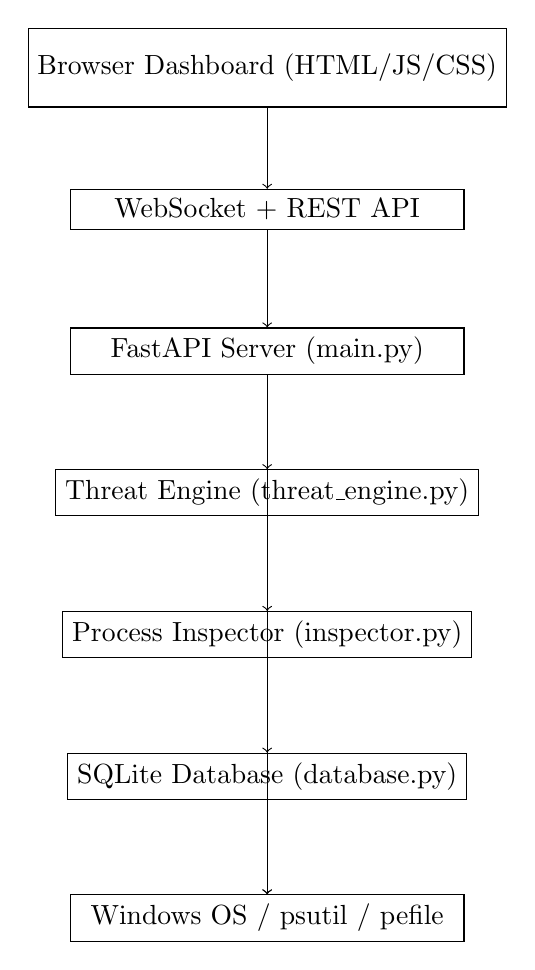
\begin{tikzpicture}[node distance=1.8cm]

\node (browser)  [rectangle, draw, minimum width=5cm, minimum height=1cm] {Browser Dashboard (HTML/JS/CSS)};
\node (ws)       [rectangle, draw, below of=browser, minimum width=5cm] {WebSocket + REST API};
\node (fastapi)  [rectangle, draw, below of=ws, minimum width=5cm] {FastAPI Server (main.py)};
\node (engine)   [rectangle, draw, below of=fastapi, minimum width=5cm] {Threat Engine (threat\_engine.py)};
\node (inspector)[rectangle, draw, below of=engine, minimum width=5cm] {Process Inspector (inspector.py)};
\node (db)       [rectangle, draw, below of=inspector, minimum width=5cm] {SQLite Database (database.py)};
\node (os)       [rectangle, draw, below of=db, minimum width=5cm] {Windows OS / psutil / pefile};

\draw[->] (browser) -- (ws);
\draw[->] (ws) -- (fastapi);
\draw[->] (fastapi) -- (engine);
\draw[->] (fastapi) -- (inspector);
\draw[->] (fastapi) -- (db);
\draw[->] (engine) -- (os);
\draw[->] (inspector) -- (os);

\end{tikzpicture}
\caption{Malviz System Architecture}
\end{figure}

\begin{figure}[H]
\centering
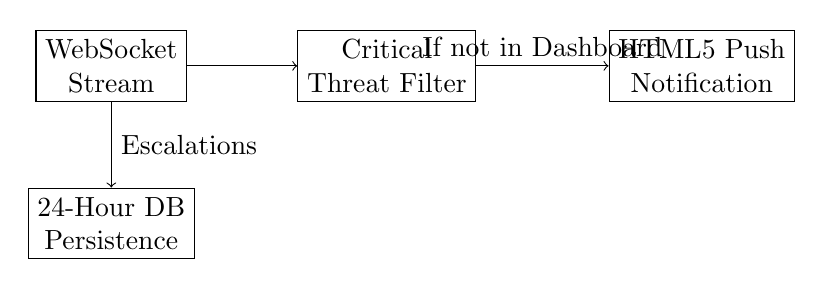
\begin{tikzpicture}[node distance=2cm, auto]
  \node (stream) [rectangle, draw, align=center] {WebSocket\\Stream};
  \node (filter) [rectangle, draw, right of=stream, node distance=3.5cm, align=center] {Critical\\Threat Filter};
  \node (notif) [rectangle, draw, right of=filter, node distance=4cm, align=center] {HTML5 Push\\Notification};
  \node (db) [rectangle, draw, below of=stream, node distance=2cm, align=center] {24-Hour DB\\Persistence};
  
  \draw[->] (stream) -- (filter);
  \draw[->] (filter) -- node {If not in Dashboard} (notif);
  \draw[->] (stream) -- node {Escalations} (db);
\end{tikzpicture}
\caption{Real-Time Alert and Escalation Tracking Workflow}
\end{figure}

\section{Backend Modules}

\subsection{Application Entry Point (main.py)}

The main module initializes the FastAPI application, mounts the static file directory, and sets up all API routes. On startup, the SQLite database is initialized. A WebSocket endpoint at \texttt{/ws} streams real-time telemetry to the dashboard every two seconds by calling \texttt{analyze\_processes()} from the threat engine. New threats are automatically logged to the database to prevent duplicate entries.

Key REST endpoints exposed by the application include:

\begin{itemize}
    \item \texttt{GET /api/history} -- retrieves previously logged threats from the database.
    \item \texttt{GET /api/inspect/\{pid\}} -- performs deep inspection of a given process.
    \item \texttt{GET /api/network} -- returns captured network packet data.
    \item \texttt{POST /api/action/\{action\}/\{pid\}} -- performs kill, suspend, or resume on a process.
    \item \texttt{GET /api/strings/\{pid\}} -- extracts printable ASCII strings from a process executable.
    \item \texttt{GET /api/dump/\{pid\}} -- generates and downloads a memory minidump of a process.
\end{itemize}

\subsection{Process Inspector (inspector.py)}

The \texttt{inspector.py} module provides deep forensic analysis for any running process given its PID. The analysis pipeline covers the following steps:

\begin{enumerate}
    \item \textbf{Memory Usage} -- The resident set size (RSS) is obtained using \texttt{psutil} and reported in megabytes.
    \item \textbf{SHA-256 Hash} -- The executable file is read from disk and hashed to verify file integrity and detect masquerading binaries.
    \item \textbf{Token Inspection} -- Windows security tokens are queried using the \texttt{win32security} API to determine the process integrity level (Low, Medium, High, or System) and list enabled privileges.
    \item \textbf{Handle Enumeration} -- Open file handles, active socket connections, and loaded DLLs are enumerated via \texttt{psutil}.
    \item \textbf{PE Static Analysis} -- The \texttt{pefile} library parses the Portable Executable structure of the process binary to extract the DOS header, NT file header, section headers, and the full import table.
    \item \textbf{Memory Minidump} -- Using \texttt{DbgHelp.MiniDumpWriteDump} via the Windows ctypes API, the module can generate a \texttt{.dmp} file for offline forensic analysis.
\end{enumerate}

The inspector also provides a \texttt{format\_hex\_dump()} helper that renders binary data in a classical hex editor format, interleaving hexadecimal values with their printable ASCII equivalents.

\subsection{Threat Detection Engine (threat\_engine.py)}

The threat engine is the core detection component of Malviz. It scans all running processes using \texttt{psutil} and applies a set of behavioral detection rules inspired by the MITRE ATT\&CK framework. Detection heuristics implemented in the engine include:

\begin{itemize}
    \item \textbf{Suspicious Execution Path} -- processes running from directories such as \texttt{Temp}, \texttt{ProgramData}, \texttt{AppData}, or \texttt{Downloads} are flagged.
    \item \textbf{Process Masquerading} -- processes whose executable name matches a known Windows system binary (e.g., \texttt{svchost.exe}, \texttt{lsass.exe}) but are located outside standard system directories are flagged as critical.
    \item \textbf{Dangerous Parent-Child Relationships (PrintNightmare Pattern)} -- processes such as \texttt{spoolsv.exe} spawning command shells like \texttt{powershell.exe} or \texttt{cmd.exe} are flagged as a known exploitation pattern.
    \item \textbf{System Shell Spawned by Unexpected Parent} -- \texttt{cmd.exe} or \texttt{powershell.exe} running under a SYSTEM account with an anomalous parent process are flagged.
    \item \textbf{LOLBin Abuse} -- use of legitimate Windows binaries such as \texttt{mshta.exe}, \texttt{wscript.exe}, \texttt{certutil.exe}, and \texttt{rundll32.exe} for potentially malicious purposes is detected.
    \item \textbf{Network Anomaly Detection} -- active connections to uncommon remote ports or external IP addresses by normally non-networked processes are flagged.
\end{itemize}

Each detection produces a structured threat record containing the PID, process name, executable path, parent process, threat severity level, reason descriptions, and associated network connections.

\subsection{Database Layer (database.py)}

The database module manages a SQLite database at the application's working directory. It provides three operations:

\begin{itemize}
    \item \texttt{init\_db()} -- creates the \texttt{suspected\_processes} and \texttt{daily\_escalations} tables if they do not already exist.
    \item \texttt{log\_threat(threat\_data)} -- inserts a new generic threat record with a UTC timestamp.
    \item \texttt{log\_escalation(escalation\_data)} -- logs specific privilege escalation pathways and automatically prunes any entries older than 24 hours to maintain a lightweight context window.
    \item \texttt{get\_history()} \& \texttt{get\_recent\_escalations()} -- retrieves the most recent threats and daily escalations dynamically.
\end{itemize}

\section{Frontend Dashboard}

The frontend is a single-page application (SPA) built with HTML5, CSS3, and vanilla JavaScript. It communicates with the backend via WebSocket for live data and the \texttt{fetch()} API for on-demand requests.

The dashboard is organized into five views:

\begin{itemize}
    \item \textbf{Overview} -- displays system resource metrics (CPU, memory, disk, network), a real-time threat severity indicator, and a list of top suspicious processes with mini sparkline charts.
    \item \textbf{Processes} -- a live, searchable table listing all running processes with their PID, user, executable path, and threat status badge, with per-row action buttons.
    \item \textbf{Network Analyzer} -- a Wireshark-style table showing captured DNS, TCP, and UDP packets with source and destination addressing and payload hex dumps.
    \item \textbf{Threat History} -- a log of previously detected threats stored in the database, showing severity, detection reason, and timestamp.
    \item \textbf{Simulation} -- a demonstration mode rendering simulated process and syscall data for training purposes without requiring a live threat.
\end{itemize}

\section{Attack Simulation Scripts}

Seven batch scripts were developed to reproduce specific attack scenarios infinitely, enabling validation of the detection engine and the manual ''Kill'' termination routines without requiring real malware samples:

\begin{table}[H]
\centering
\begin{tabular}{|l|l|l|}
\hline
\textbf{Script} & \textbf{Simulated Technique} & \textbf{Expected Severity} \\
\hline
test\_01\_masquerading.bat & svchost.exe masquerade in Temp & Critical \\
test\_02\_printnightmare.bat & spoolsv.exe spawning powershell.exe & Critical \\
test\_03\_obfuscated\_cmdline.bat & powershell bypassing execution policy & Warning/Critical \\
test\_04\_uac\_bypass\_com.bat & fodhelper.exe spawning cmd.exe & Critical \\
test\_05\_dll\_hijack.bat & rundll32 proxy execution & Warning/Critical \\
test\_06\_impersonation\_tool.bat & PrintSpoofer token theft & Critical \\
test\_07\_scheduled\_task.bat & cmd.exe as SYSTEM via Task Scheduler & Critical \\
\hline
\end{tabular}
\caption{Attack Simulation Scripts and Expected Detections}
\end{table}

Each script initiates a harmless system binary in an infinite processing loop from a suspicious path, or manipulates execution arguments, requiring manual intervention or UI-based termination.

\section{Technology Stack}

\begin{table}[H]
\centering
\begin{tabular}{|l|l|}
\hline
\textbf{Component} & \textbf{Technology} \\
\hline
Backend Framework & FastAPI (Python) \\
ASGI Server & Uvicorn \\
Process Data & psutil \\
PE Analysis & pefile \\
Windows API & pywin32 (win32security, win32api) \\
Database & SQLite3 \\
Frontend & HTML5, CSS3, Vanilla JavaScript \\
Charts & Chart.js \\
Real-time Communication & WebSocket \\
\hline
\end{tabular}
\caption{Malviz Technology Stack}
\end{table}

\section{Summary}

This chapter described the complete design and implementation of the Malviz system. The backend is organized into four focused modules: the FastAPI application server, the deep process inspector, the behavioral threat detection engine, and the SQLite database layer. The frontend SPA provides five interactive views covering live monitoring, network analysis, threat history, and simulation. Attack simulation scripts allow controlled testing of the detection engine against representative threat scenarios without requiring live malware. Together, these components form a cohesive and extensible real-time threat monitoring platform suited for security research and education.
